%\special{pdf:encrypt ownerpw (abc) userpw (xyz) length 128 perm 2052}
\documentclass{article}
\usepackage{indentfirst}
\usepackage{enumitem}
\usepackage{graphicx}
\usepackage{amssymb}
\usepackage{tcolorbox}
\usepackage{framed}
\usepackage{array}
\usepackage{multirow}
\usepackage{tabularx}
\usepackage{booktabs}
\usepackage{tabu}
\usepackage{TikZ}
\usepackage{parskip}

\usepackage{hyperref}
\hypersetup{
    colorlinks=true,
    linkcolor=green,
    filecolor=magenta,
    urlcolor=cyan,
}

\usepackage[a4paper, margin=2in]{geometry}
\geometry{
 a4paper,
 total={210mm,297mm},
 left=20mm,
 right=20mm,
 top=20mm,
 bottom=20mm,
 }


\usepackage{xcolor,lipsum}
\usepackage{background}

%-------------------------------------------------------------------------------------
%SIDE BORDER FRAME

\usetikzlibrary{calc}
\SetBgScale{1}
\SetBgAngle{0}
\SetBgColor{black}
\SetBgContents{
	
\begin{tikzpicture}[overlay,remember picture]
	\draw [line width=1pt,rounded corners=7pt,
	]
	($ (current page.north west) + (1.5cm,-1cm) $)
	rectangle
	($ (current page.south east) + (-1cm,1cm) $);
	\draw [line width=1pt,rounded corners=7pt];
	\end{tikzpicture}
}
%-----------------------------------------------------------------------------
\usepackage{setspace}

%--------------------------------------------
%FOR MURGED COLUMNS INTO ONE COLUMN
\newcommand{\specialcell}[2][c]{%
  \begin{tabular}[#1]{@{}c@{}}#2\end{tabular}}

\author{Vaibhav}

%--------------------------------------------------------------------------------------
%--------------------------------------------------------------------------------------


\begin{document}
\pagestyle{empty}
\linespread{1.5}
%----------------------------------------------------------------------------------------------------------------------%%
%                                                  Header
\begin{minipage}{\textwidth}
	
	\begin{tabular}{ l r}
		\begin{minipage}{0.75\textwidth}
			\begin{flushleft}
				{ \tabulinesep=1.2mm
				\def\arraystretch{1.5}
				\begin{tabular}{lcl}
				\multicolumn{3}{l}{{\textbf{KUMBHAR VAIBHAV ANANDA}}}	\\
				\multicolumn{3}{l}{{{Flat No-11, Silver Oak Park,}}}	\\
				\multicolumn{3}{l}{{{MSEB Road, Vishrambaag,}}}	\\
				\multicolumn{3}{l}{{{Sangli - 416416}}}	\\
				Mobile No & : & +91-9403183440\\
				 
				Email-Id & : & \href{mailto:vkumbhar94@gmail.com}{vkumbhar94@gmail.com}\\

				\end{tabular} }
			\end{flushleft}
		\end{minipage}
		&
		\begin{minipage}{0.25\textwidth}
%			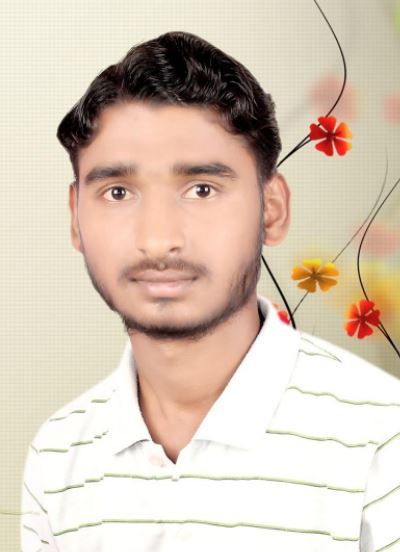
\includegraphics[width=0.8\textwidth]{Vaibhav.jpg}
			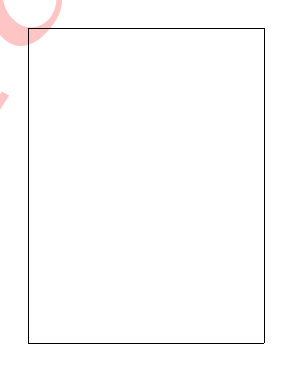
\begin{tikzpicture}
				\draw (-1.5,2) -- (1.5,2);
				\draw (-1.5,-2) -- (1.5,-2);
				\draw (-1.5,2) -- (-1.5,-2);
				\draw (1.5,2) -- (1.5,-2);
			\end{tikzpicture}
		\end{minipage}
	\end{tabular}\\
\end{minipage}

\vspace{1cm}
%----------------------------------------------------------------------------------------------------------------%%%
%                                        Career objective
%\begin{tcolorbox}
\begin{minipage}{\textwidth}

\begin{framed}
	\large{\textbf{CAREER OBJECTIVE}}
\end{framed}
%\end{tcolorbox}
	\large{\textup{\setlength{\parindent}{15pt}
			\indent I am looking for an opportunity in a reputed organization which will help me deliver my best and upgrade my skills in engineering and meet the demands of
			the organization.}}


\end{minipage}
\vspace{1cm}
%---------------------------------------------------------------------------------------------------------------------------
%                                      Engineering Qualification

\begin{minipage}{\textwidth}

\begin{framed}
	\large{\textbf{ENGINEERING QUALIFICATION}}
\end{framed}
\large{\textbf{\setlength{\parindent}{15pt}
		\indent Branch: Computer Science and Engineering}}

\begin{flushleft}

\setlength{\tabcolsep}{0.7em}
\def\arraystretch{1.5}
\begin{tabular}{|p{\dimexpr.19\textwidth} |>{\centering\arraybackslash} p{\dimexpr.33\textwidth-3\tabcolsep} |p{\dimexpr.19\textwidth-3\tabcolsep} |
		p{\dimexpr.16\textwidth-3\tabcolsep} | p{\dimexpr.16\textwidth-3\tabcolsep}|}
	\hline
	\centering\textbf{CLASS} & \centering\textbf{INSTITUTE} & \centering\textbf{SEM-I} & \centering\textbf{SEM-II} & \textbf{YEAR}\\
	\hline
	\centering Final Year &  \multirow{3}{*}{ \specialcell{Walchand College \\ Of Engineering, Sangli}} & \multicolumn{2}{c|}{Pursuing} & 2015-16\\
	\cline{1-1}\cline{3-5}
	\centering Third Year&  & \centering 8.21 & \centering 8.08 &  2014-15 \\
	\cline{1-1}\cline{3-5}
	\centering Second Year&  & \centering 7.48 & \centering 7.52 &  2013-14 \\
	\cline{1-1}\cline{3-5}
	\centering First Year & & \centering  7.28 & \centering 7.38 & 2012-13 \\
	\hline
\end{tabular}
\end{flushleft}
\vspace{0.3cm}

\begin{flushright}
	Cummulative CPI : {\textbf{7.66}}
\end{flushright}


\end{minipage}
\vspace{1cm}
%----------------------------------------------------------------------------------------------------------------------------------
%				Pre-Engineering Qualification

\begin{minipage}{\textwidth}
\begin{framed}
	\large{\textbf{PRE-ENGINEERING QUALIFICATION}}
\end{framed}
\begin{flushleft}
\setlength{\tabcolsep}{0.7em}
\def\arraystretch{1.5}
\begin{tabular}{|p{\dimexpr.17\textwidth} | p{\dimexpr.35\textwidth-3\tabcolsep} |p{\dimexpr.17\textwidth-3\tabcolsep} |
		p{\dimexpr.17\textwidth-3\tabcolsep} | p{\dimexpr.17\textwidth-3\tabcolsep}|}
	\hline
\centering\textbf{EXAM} & \centering\textbf{ INSTITUTE} & \centering\textbf{BOARD} & \centering\textbf{MARKS}& \textbf{YEAR}\\
	\hline
	\centering H.S.C. & \specialcell{  Karmveer Bhaurao Patil\\ Mahavidyalaya, Pandharpur}  & \multirow{2}{*}{ \specialcell{PUNE}} & \centering 83.33 & \specialcell{ 2011-12}\\
	\cline{1-2}\cline{4-5}
	\centering S.S.C. & \centering Hanuman Vidya Mandir, Marawade &  & \centering 91.45 & 2009-10 \\
	\hline
\end{tabular}
\end{flushleft}
\vspace{0.3cm}
\begin{flushright}
	MHT-CET : {\textbf{143}}
\end{flushright}

\end{minipage}

\vspace{1cm}




%-----------------------------------------------------------------------------
%AREAS OF INTEREST
\begin{minipage}{\textwidth}
	\begin{framed}
		\large{\textbf{AREAS OF INTEREST}}
	\end{framed}
	\begin{itemize}
		\item Database Management System
		\item Programming in Java
	\end{itemize}
\end{minipage}

\vspace{1cm}
%----------------------------------------------------------------------------------------------------------------------------------
%				Technical Skills
\begin{minipage}{\textwidth}
\begin{framed}
	\large{\textbf{TECHNICAL SKILLS}}
\end{framed}
\setlength{\tabcolsep}{0.7em}
\def\arraystretch{1.7}
\begin{tabular}{lcp{0.5\textwidth}}
	Languages & : & Core Java,C, C++, PL-SQL, Python (Novice)\\
	Operating System &  : &  Windows 8, Ubuntu- 13.04/14.10 (Novice)\\
	Development Tools &  : & IntelliJ Idea 14.0.1, Eclipse, Visual Studio 2013(Novice)\\
	Technologies &  : &  Django (Novice), Android (Novice)\\
	Versioning Control Tools & : & Git\\
	Documentation Tools & : & Latex, Microsoft word 13\\

\end{tabular}
\end{minipage}

\vspace{1cm}


%----------------------------------------------------------------------------------------------------------------------------------
%				Projects Undertaken
\begin{minipage}{\textwidth}

\begin{framed}
	\large{\textbf{PROJECTS UNDERTAKEN}}
\end{framed}
\vspace{0.1cm}
\begin{comment}

\begin{itemize}
	\itemsep1pt \parskip0pt \parsep0pt
	\setlength{\itemsep}{0.1cm}%
	\setlength{\parskip}{0.2cm}%

	\item{
		\textbf{\large{A Technical Forum }}ease to solve technical Queries of students
		\begin{itemize}
			\item[$\circ$] {Duration : 3 Months}
			\item[$\circ$] {Team : 3 Members}
			\item[$\circ$] {My Role : Database backend design and implementation}
		\end{itemize}
	\textbf{Description:}\\
		\setlength{\parindent}{15pt}
		\indent This Project done by using \textbf{Django web Framework} which is written in python.
	}
\end{itemize}

\end{comment}


%\begin{comment}

\setlength{\tabcolsep}{0.1em}
\def\arraystretch{1.7}
\begin{center}
\begin{tabularx}{\linewidth}{|X|X|X|}
	\hline
	 \centering\textbf{ TITLE} & \centering\textbf{DESCRIPTIOIN} & \textbf{TECHNOLOGY USED}\\
\hline 
	\centering 
		Augmented Reality System for Exploring the College campus
 	&
	\centering Ease to get Information of College's All Departments, Labs and Library. 
	&
	\begin{itemize}
		\item Augmented Reality SDK
		\item Android
	\end{itemize}\\
	\hline

	\centering A Technical Forum  & Ease to solve technical Queries of students &
	\begin{itemize}
		\item Django with Python
		\item Bootstrap
	\end{itemize} \\
	\hline
\end{tabularx}
\end{center}
%\end{comment}

\end{minipage}	


\vspace{1cm}
	

%----------------------------------------------------------------------------------------------------------------------------------
%				WORKSHOP ATTENDED
\begin{comment}

\begin{framed}
	\large{\textbf{WORKSHOP ATTENDED}}
\end{framed}

\begin{itemize}
	\item Attended workshop on \textbf{"Hadoop Basics"} in March 2015 by "Mr. Kapil Bhosale".
	\item Attended workshop on \textbf{"Ruby on rails Workshop"} by Sushant Mane.
	\item Attended workshop on \textbf{"Clean Coding and Object Oriented Design"} by \textbf{"Thaughtworks"}. 
\end{itemize}


\vspace{1cm}
%----------------------------------------------------------------------------------------------------------------------------------
%				CO-CURRICULAR ACTIVITIES
\begin{framed}
	\large{\textbf{CO-CURRICULAR ACTIVITIES}}
\end{framed}
\begin{itemize}
	\item Winner in \textbf{"Code Marathon"} in \textbf{"Vision 2014"}.
	\item Runner up in \textbf{"Code Trix"}  by \textbf{ "SAIT Club"}.
\end{itemize}


\vspace{1cm}
\end{comment}


%--------------------------------------------------------------------------------------------
%						Achievements and accolades
\begin{minipage}{\textwidth}
	\begin{framed}
		\large{\textbf{ACHIEVEMENTS AND ACCOLADES}}
	\end{framed} 
	\begin{comment}
	\large{\textbf{\setlength{\parindent}{15pt}
			\indent Coding Competitions}}\\
	\end{comment}
	\begin{itemize}
		\item Winner of an event \textbf{"Code Marathon"} Coding Competition in C language organized by \textbf{"VISION 2k14"}.
		\item Winner of an event \textbf{"D-Softa"} Coding Competition in C language organized by \textbf{"CODE WAR-2k13"}.
		\item Runner up in an event \textbf{"Reverse Trix"}  by \textbf{ "SAIT Club"}.
		\item Honored with \textbf{"Adarsh Vidhyarthi Purskar"} in 9th standard by My School \textbf{"Hanuman Vidya Mandir"}
	\end{itemize}
\end{minipage}




\vspace{1cm}
%----------------------------------------------------------------------------------------------------------------------------------
%				EXTRA-CURRICULAR ACTIVITIES

\begin{minipage}{\textwidth}
	
\begin{framed}
	\large{\textbf{EXTRA-CURRICULAR ACTIVITIES}}
\end{framed}

\textbf{\setlength{\parindent}{20pt}\indent Association of Computer Science and Engineering Students (ACSES)}
\begin{itemize}
	\itemsep1pt \parskip0pt \parsep0pt
	\setlength{\itemsep}{0.1cm}%
	\setlength{\parskip}{0.2cm}%
	\setlength{\parsep}{0.2cm}%
	\item Appointed as \textbf{Program director} of \textbf{ACSES} a leading students organization in WCE, Sangli for the year 2014-2015.
	\item Organized Social Event \textbf{SITAC 2k15 (Social IT Awareness Campaign)} by \textbf{ACSES} on Computer Technology and Introduction to Computer”.
	\item Worked as \textbf{Coordinator} of \textbf{ACSES}, member of committee of \textbf{TECHUMEN 2k13}
	\item Contributed in \textbf{SITAC 2k13}
	
\end{itemize}

\end{minipage}

\vspace{1cm}






%---------------------------------------------------------------------------------------------------------------------------------
%					Strengths
\begin{minipage}{\textwidth}
	\begin{framed}
		\large{\textbf{STRENGTHS}}
	\end{framed}
	\begin{itemize}
		\item Hard working and full dedication to my work.
		\item Ability to adapt with new technology and programming language.
	\end{itemize}		
\end{minipage}



%----------------------------------------------------------------------------------------------------------------------------------
%				HOBBIES
\begin{comment}

\begin{framed}
	\large{\textbf{HOBBIES}}
\end{framed}
\begin{itemize}
	\item Coding
	\item Learning New Technologies.
	\item Daily Workout.
	\item Listening Songs.
\end{itemize}


\end{comment}
\vspace{1cm}

%--------------------------------------------------------------------------------------------------------------------------
%                                    Personal Details
\begin{minipage}{\textwidth}
\begin{framed}
	\large{\textbf{PERSONAL DETAILS}}
\end{framed}
\def\arraystretch{1.5}
\begin{tabular}{lcm{0.5\linewidth}}
	{Father's Name} & :& Mr. Ananda Kumbhar\\
	{Mother's Name} & :& Mrs. Minakshi Kumbhar\\
	{Date of Birth} & : & 12 Oct, 1994\\
	{Sex/Status} & : & Male/Single\\
	{Nationality} & : & Indian\\
	\begin{comment}

	{Local Address} & : & Flat No: 11, Silver Oak Park, MSEB Road, Vishrambag, 
	Sangli-416415\\
	\end{comment}	
	{Permanent Address} & : & 181, Kumbhar Wasti, Marawade, Mangalwedha,  Solapur- 413319\\

	{Languages known} & : &  English, Hindi, \underline{\textbf{Marathi}}.\\
	{Hobbies} & : & Gymnastics, Listening Songs.\\
\end{tabular}


\end{minipage}
\vspace{1cm}
%----------------------------------------------------------------------------------------------------------------------------------
%				DECLARATION

\begin{minipage}{\textwidth}
\begin{framed}
	\large{\textbf{DECLARATION}}
\end{framed}
	\large{\setlength{\parindent}{15pt} \indent I hereby declare that all the information provided above is true to the best of my knowledge. }


\vspace{3cm}
\begin{tabular}{cc}
\begin{minipage}{0.5\textwidth}
\begin{flushleft}Place:
\end{flushleft}
\end{minipage}
&
\begin{minipage}{0.5\textwidth}
\begin{center}Signature:
\end{center}
\end{minipage}
\end{tabular}


\begin{tabular}{cc}
\begin{minipage}{0.5\textwidth}
\begin{flushleft}Date:
\end{flushleft}
\end{minipage}
&
\begin{minipage}{0.5\textwidth}
\begin{center} (Kumbhar Vaibhav A.)
\end{center}
\end{minipage}
\end{tabular}

\end{minipage}

\end{document}